\documentclass[10pt,twocolumn,letterpaper]{article}

\usepackage{cvpr}
\usepackage{times}
\usepackage{epsfig}
\usepackage{graphicx}
\usepackage{amsmath}
\usepackage{amssymb}
\usepackage[table,xcdraw]{xcolor}
\usepackage{subfig}
\usepackage{caption}
\usepackage{subcaption}

% Include other packages here, before hyperref.

% If you comment hyperref and then uncomment it, you should delete
% egpaper.aux before re-running latex.  (Or just hit 'q' on the first latex
% run, let it finish, and you should be clear).
\usepackage[pagebackref=true,breaklinks=true,letterpaper=true,colorlinks,bookmarks=false]{hyperref}

\cvprfinalcopy % *** Uncomment this line for the final submission

\def\cvprPaperID{****} % *** Enter the CVPR Paper ID here
\def\httilde{\mbox{\tt\raisebox{-.5ex}{\symbol{126}}}}

% Pages are numbered in submission mode, and unnumbered in camera-ready
% \ifcvprfinal\pagestyle{empty}\fi
\begin{document}

%%%%%%%%% TITLE
\title{Real Time Flying Object Detection: CS 7643}

\author{Dillon Reis*, Jordan Kupec*, Jacqueline Hong*, Ahmad Daoudi*\\
Georgia Institute of Technology\\
{\tt\small dreis7@gatech.edu, jkupec3@gatech.edu, jhong356@gatech.edu, adaoudi3@gatech.edu}
% For a paper whose authors are all at the same institution,
% omit the following lines up until the closing ``}''.
% Additional authors and addresses can be added with ``\and'',
% just like the second author.
% To save space, use either the email address or home page, not both
}

\maketitle
%\thispagestyle{empty}

%%%%%%%%% ABSTRACT
\begin{abstract}
   This project presents a model for inference of a wide array of flying objects in real-time. 
   This remains challenging due to large variance of the object scales during inference, object rate of speed, 
   and low variance between a subset of classes. These findings can then be used for reference/further research 
   regarding object detection by remote digital airport towers, unmanned aerial vehicles (UAVs), or any surveillance 
   systems utilizing optical data. To address some of the presented challenges, we utilize the current state of the art 
   single-shot detector, YOLOv8, in an attempt to find the best trade-off between inference speed and mAP. RESULTS TBD
\end{abstract}

%%%%%%%%% BODY TEXT
\section{Introduction/Background/Motivation}
It is no surprise that drones and mini-UAVs still remain an integral part of modern warfare. They present a stealth capability 
and can avoid detection by radar due to their small electromagnetic signature. They are also small, highly maneuverable, and 
omit low levels of noise. While methods such as utilizing radio and acoustic detection have been proposed as countermeasures, they 
are currently known to be inaccurate. This motivates the integration of a visual detector in any such detection system.\\
Use cases (WIP): flying regulation enforcement (ie. must be a min distance between other aircraft), wireless communication, drug delivery (reference prison use case), mapping areas (reference mapping the Mojave Desert with drones), suicide drones (reference recent Ukraine news)\\
The primary objective of this project is to provide a model that detects a wide array of flying objects in real-time with the latest 
state-of-the-art single-shot detector YOLOv8. These results can be used as a reference for further research by remote digital airport 
towers to detect aerial threats to a runway, surveillance systems for drone detection, and UAVs and for aircraft detection/threat identification. 
While YOLOv8 is being regarded as the new state-of-the-art, an official paper has yet to be released. This motivates our secondary objective, 
which is to explain the new architecture and functionality that YOLOv8 has adapted.\\
(5 points) What did you try to do? What problem did you try to solve? Articulate your objectives using absolutely no jargon. 

[Still add stuff to the various use case examples above later, but focusing on:]
    
We're going to be focusing on a recent event where people used drones to surveil U.S. Border Patrol agents in order to smuggle migrants. Subsequent investigation led the agents to find the footage that the smugglers recorded. They already have towers that use object detection for people and motor vehicles, but not drones (to the best of our knowledge) [SOURCE]. "With dense vegetation and vast tracts of isolated ranch land, the region attracts the human and drug smugglers to try their chances." This can be tied to the varying background challenge - how drones would blend in and can possibly not get detected. Basically, they say that the technology on their digital towers is state-of-the-art, but it seems to focus on finding illegal migrants only. \\
With drones becoming so accessible now, they need to be able to detect that too, but the landscape/background makes it a challenge. Other challenges are that the drones will be very small in the footage because people won't want to fly near the digital towers. This is how we tie in the size issue. Third, there is also the challenge of other flying objects coming into view. There will be birds and it's important to distinguish between a bird and a drone. We can also see how we do against the Drone-vs-Bird dataset. There will also be other aircraft flying across the border or within the field of view, so it's important for us to be able to distinguish those from drones too. Note that other flying object detection projects are very focused on UAVS, specifically Drone-vs-Bird. This is not a reflection of real-world conditions. Selecting these challenges leads to having a model that will perform better for real-world use cases. Unlike previously published models, tackling these challenges gives our model the variance needed for real-world applications.\\
The overall problem is to be able to provide a model that detects a wide array of flying objects in real time with the latest state-of-the-art single-shot detector, YOLOv8. Our objectives relate to the challenges that come with our domain (which are also the common challenges of object detection on UAVs).\\

(5 points) How is it done today, and what are the limits of current practice?
Currently, single-stage detectors are the de-facto architecture choice for fast inference speeds. This choice comes at the expense of exchanging the higher accuracy you would typically expect from a two-state detector for the speed of a single-stage detector. Real-time object detection remains challenging due to variances in object spatial sizes and aspect ratios, inference speed, and noise. This is especially true for our use case, as flying objects can change location, scale, rotation, and trajectory very quickly. This conveys the necessity for fast inference speed (which for the purpose of this project is between 30 - 60 fps on 1080p video feed). \\

(5 points) Who cares? If you are successful, what difference will it make? 
If we are successful, this will make a difference in the realm of object detection, where we will be able to provide more novel insight related to our challenges with our results and observations from our experiments trying to solve the landscape (variance/blending), size, and other flying objects challenges. In addition, this will positively affect the world of surveillance due to our focus on real-world conditions and use cases. Drones are capable of much danger and harm, and we can make the world a safer place. Surveillance technology needs to adapt quickly because drone use is increasing at an alarming rate.\\

(5 points) What data did you use? Provide details about your data, specifically choose the most important aspects of your data mentioned \href{https://arxiv.org/abs/1803.09010}{here}. You don’t have to choose all of them, just the most relevant.

Jackie: Didn't realize this section requires some extra reading (https://arxiv.org/pdf/1803.09010.pdf). Still reading and filling out this info based on the paper.
%-------------------------------------------------------------------------
%------------------------------------------------------------------------
\section{Approach}
We chose the YOLOv8 architecture under the assumption that it would provide us the highest probability of success given the task. YoloV8 is 
assumed to be the new state-of-the-art due to its higher mAPs and lower inference speed on the COCO dataset. However, an official paper has 
yet to be released. It also specifically performs better of aerial objects, which is the scope of this project. We utilized the code repository 
from Ultralytics. We decide to implement transfer learning and initialize our models with pre-trained weights to then begin training on the 
custom data set. These weights are from a model trained on the COCO dataset. Due to only having access to a single NVIDIA RTX 3080 and 3070, 
a greedy model selection/hyper-parameter tuning approach was chosen. We first train a version of the small,medium, and large versions of the 
model with default hyper-parameters for 100 epochs. Then, we decide which model is optimal for our use case given the trade off between inference 
speed and mAP-50-95 on the validation set. After model size is selected, a greedy hyper-parameter search is conducted with 10 epochs per each 
set of hyper-parameters. Finally, the model with the optimal hyper-parameters trains for 163 epochs to generate the final model.
Due to the large class imbalance, poor performance on the validation set was anticipated on the minority classes. However, this was not observed.

\subsection{Model Choice and Evaluation}

We evaluate small,medium, and large versions of the models to determine an optimal trade-off between inference speed and mAP50-95 to then optimize the hyper-parameters. The small, medium, and large models have (11151080, 25879480, \& 43660680) parameters and (225,295, \& 365) layers respectively. After training the models we see there is a noticeable increase in mAP50-95 between small and medium models (0.05), but not much delta between medium and large (0.002). We also see that small, medium, and large infer at 4.1,5.7, and 9.3 milliseconds respectively on the validation set containing 640 x 640 images. However, our original goal is to reach an average inference speed between 30 to 60 frames for 1080p. When testing the medium-size model on multiple 1080p HD videos, we observe an average total speed (pre-process speed(0.5ms) + inference speed(17.25ms) + post-process speed(2ms)) of 19.75 ms (50 frames per second), which aligns with our primary objective. This leads to our selection of the medium-size model to begin tuning hyper-parameters.

Due to a lack of computational resources, we evaluate only 10 epochs for each small set of hyper-parameters as an indicator for potential performance with more epochs. We observe that this assumption was correct, as training with the optimal set of hyper parameters achieves better performance at epoch 100 compared to default hyper-parameters (0.027)\ref{fig:YOLOv8_mAP50-95_val}. This takes around 35 minutes per every combination. After evaluating mAP50-95 on the validation set after 10 epochs, the following hyper-parameters are chosen:
\begin{itemize}
  \item Batch Size : 16
  \item Optimizer : Stochastic Gradient Descent (SGD).
  \item Initial/Final Learning Rate : 0.01
  \item Momentum : 0.937
  \item Weight Decay : 0.01
  \item Classification Loss Weight : 1
  \item Box Loss Weight : 5.5
  \item Distribution Focal Loss Weight : 2.5
\end{itemize}

\begin{figure*}[h]
    \centering
    \subfloat[\centering Confusion matrix for all classes \label{
    Confusion matrix for all classes
    }]{{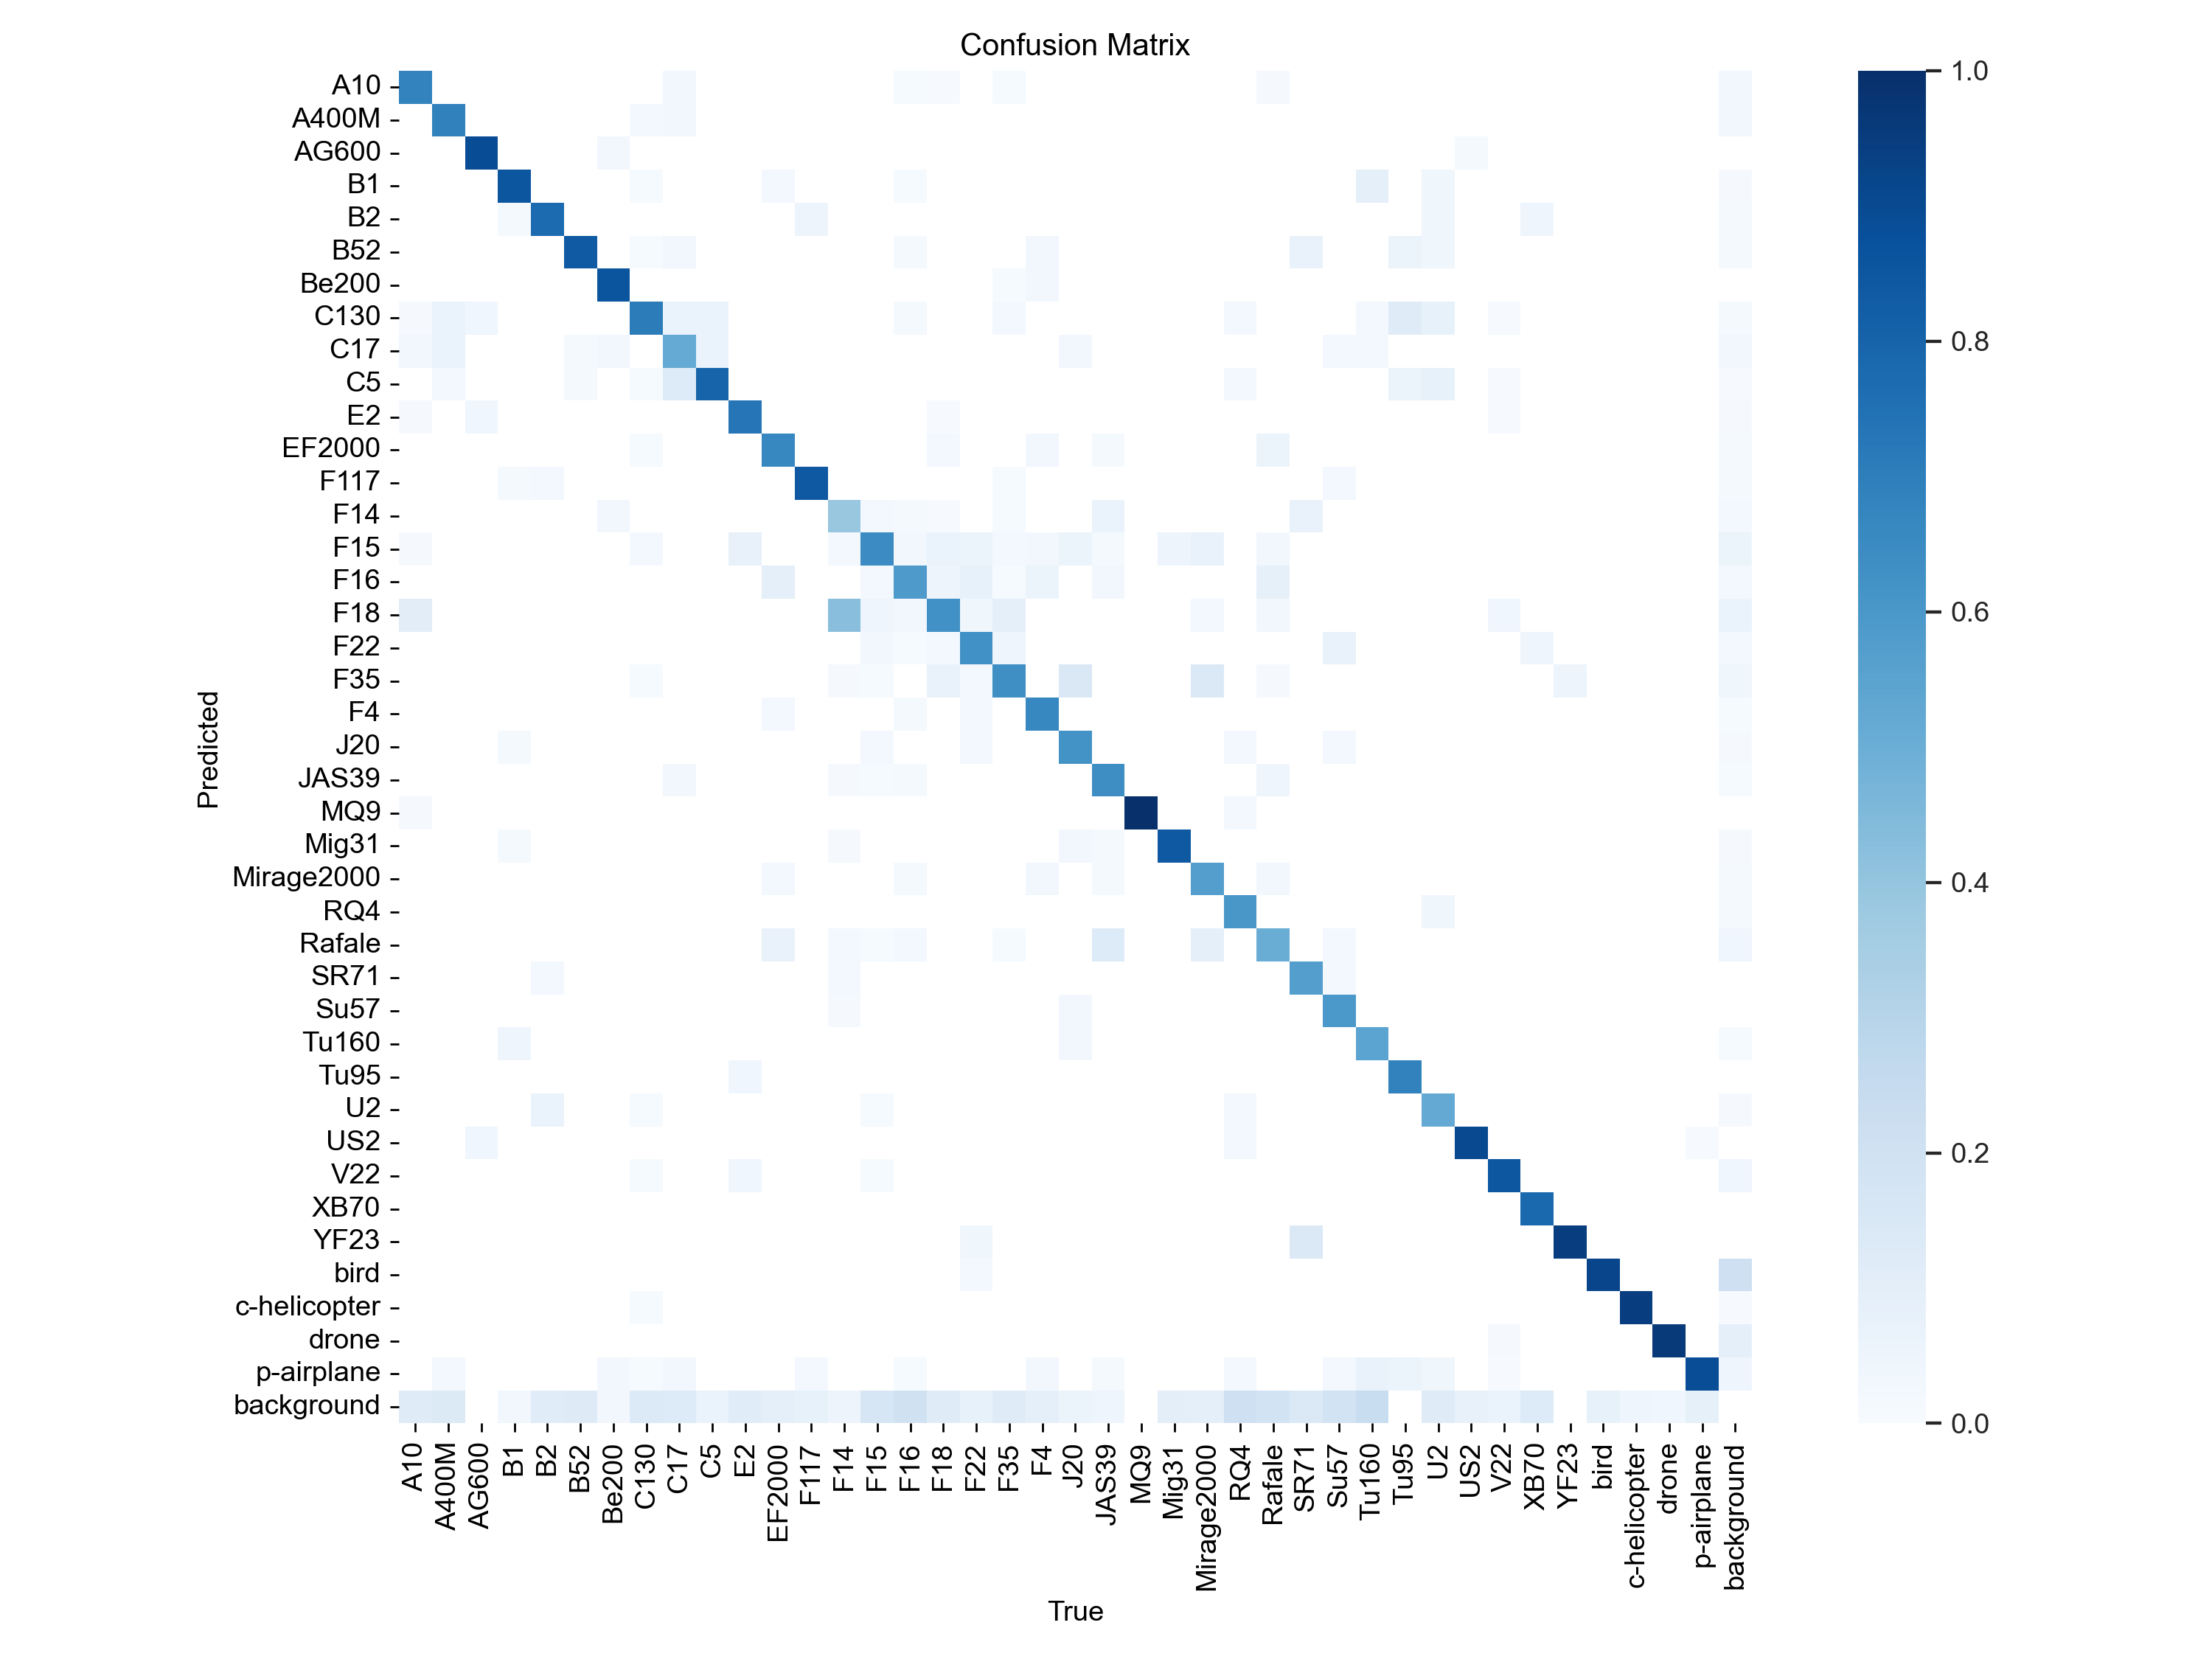
\includegraphics[width=9.5cm,height=7cm]{figures/confusion_matrix.png}}}
    \qquad
    \subfloat[\centering YOLOv8 validation mAP50-95 \label{YOLOv8_mAP50-95_val}]{{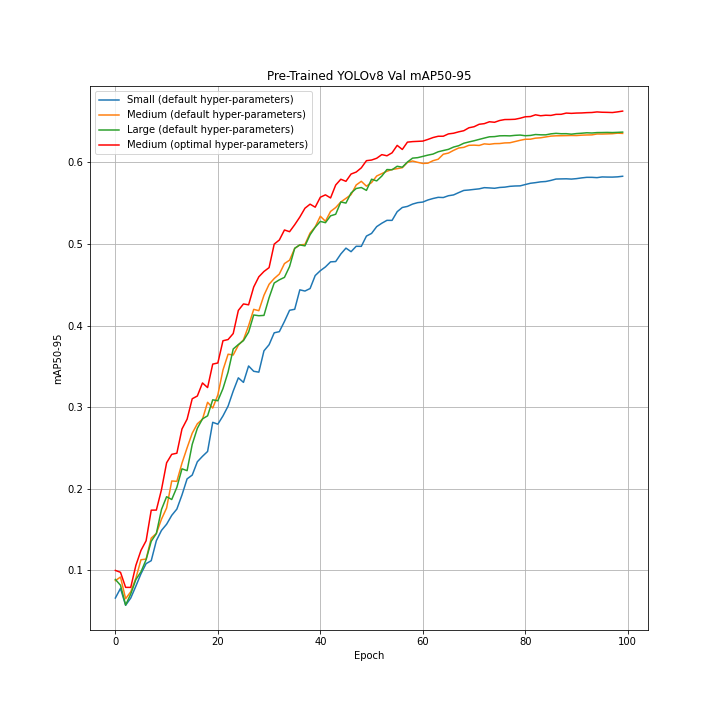
\includegraphics[width=7cm,height=7.9cm]{figures/Pre-Trained YOLOv8 Val mAP50-95.png} }}%
    \caption{YOLOv8 Validation}%
    \label{fig:Model_Evaluation}
\end{figure*}


After training for 163 epochs we achieve an mAP50-95 of 0.685 and recall of 0.792.

\begin{multline}
\lambda_{coord}\sum_{i=0}^{S^2}\sum_{j=0}^{B}\mathbf{1}_{ij}^{obj}\Big[(x_i-\hat{x}_i)^2+(y_i-\hat{y}_i)^2\Big] \\ + \lambda{coord}\sum_{i=0}^{S^2}\sum_{j=0}^{B}\mathds{1}_{ij}^{obj}\Big[(\sqrt{w_i}-\sqrt{\hat{w}_i})^2+(\sqrt{h_i}-\sqrt{\hat{h}_i})^2\Big]\\
+\sum_{i=0}^{S^2}\sum_{j=0}^{B}\mathds{1}_{ij}^{obj}(C_i-\hat{C}i)^2\\
+\lambda{noobj}\sum_{i=0}^{S^2}\sum_{j=0}^{B}\mathds{1}_{ij}^{noobj}(C_i-\hat{C}i)^2\\
+\sum_{i=0}^{S^2}\mathds{1}_{i}^{obj}\sum_{c\in classes}(p_i(c)-\hat{p}_i(c))^2
\end{multline}
	  


\section{Experiments and Results}

(10 points) How did you measure success? What experiments were used? What were the results, both quantitative and qualitative? Did you succeed? Did you fail? Why? Justify your reasons with arguments supported by evidence and data.

\textbf{Important: This section should be rigorous and thorough. Present detailed information about decision you made, why you made them, and any evidence/experimentation to back them up. This is especially true if you leveraged existing architectures, pre-trained models, and code (i.e. do not just show results of fine-tuning a pre-trained model without any analysis, claims/evidence, and conclusions, as that tends to not make a strong project). }

%-------------------------------------------------------------------------
\section{Other Sections}


You are welcome to introduce additional sections or subsections, if required, to address the following questions in detail. 

(5 points) Appropriate use of figures / tables / visualizations. Are the ideas presented with appropriate illustration? Are the results presented clearly; are the important differences illustrated? 

(5 points) Overall clarity. Is the manuscript self-contained? Can a peer who has also taken Deep Learning understand all of the points addressed above? Is sufficient detail provided? 

(5 points) Finally, points will be distributed based on your understanding of how your project relates to Deep Learning. Here are some questions to think about: 

What was the structure of your problem? How did the structure of your model reflect the structure of your problem? 

What parts of your model had learned parameters (e.g., convolution layers) and what parts did not (e.g., post-processing classifier probabilities into decisions)? 

What representations of input and output did the neural network expect? How was the data pre/post-processed?
What was the loss function? 

Did the model overfit? How well did the approach generalize? 

What hyperparameters did the model have? How were they chosen? How did they affect performance? What optimizer was used? 

What Deep Learning framework did you use? 

What existing code or models did you start with and what did those starting points provide? 

Briefly discuss potential future work that the research community could focus on to make improvements in the direction of your project's topic.
%-------------------------------------------------------------------------

\section{Model Architecture}

With the publication of “You Only Look Once: Unified, Real-Time Object Detection” in 2015, one of the most popular object detection algorithms, YOLOv1, was first described as having a “refreshingly simple” approach. At its inception, YOLOv1 could process images at 45 fps, while a variant, fast YOLO, could reach upwards of 155 fps. It also achieved high mAP compared to other object detection algorithms at the time. \\
The main idea of YOLO is to frame the problem of object detection as a one-pass regression problem, YOLOv1 comprises a single neural network, predicting bounding boxes and associated class probability in a single evaluation. The base model of YOLO works by first dividing the input image into an S x S grid where each grid cell (i,j) predicts B bounding boxes and a confidence score for each box. The final output will be a tensor of shape: S x S x (B x 5 + C), where C is the number of categories.
\subsection{YOLOv1 Overview}

\begin{figure}[h]
    \centering
    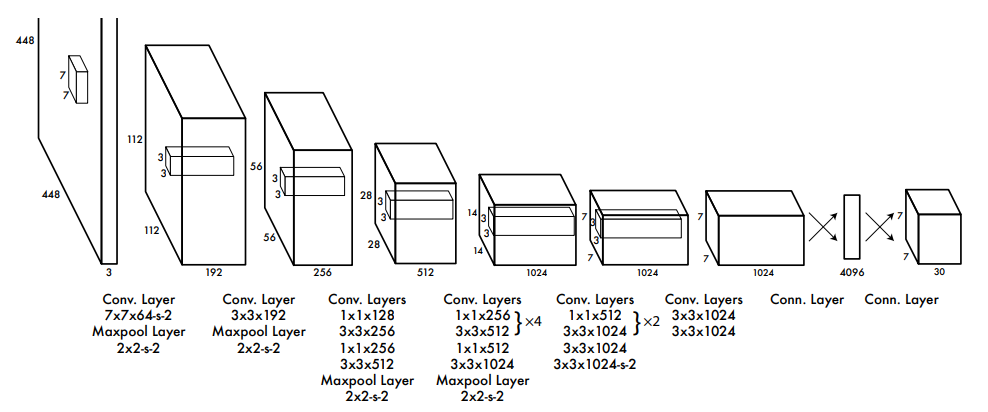
\includegraphics[width=0.4\textwidth]{figures/YOLOv1 Architecture.png}
    \caption{YOLO Architecture `\cite{YOLO_OG}}
    \label{fig:my_label}
\end{figure}

YOLOv1 architecture consists of 24 convolutional layers followed by two fully connected layers. In the paper, the authors took the first 20 convolutional layers from the backbone of the network and, with the addition of an average pooling layer and a single fully connected layer, where it was pre-trained and validated on the ImageNet 2012 dataset. During inference, the final four layers and 2 FC layers are added to the network; all initialized randomly.
\begin{figure}[h]
    \centering
    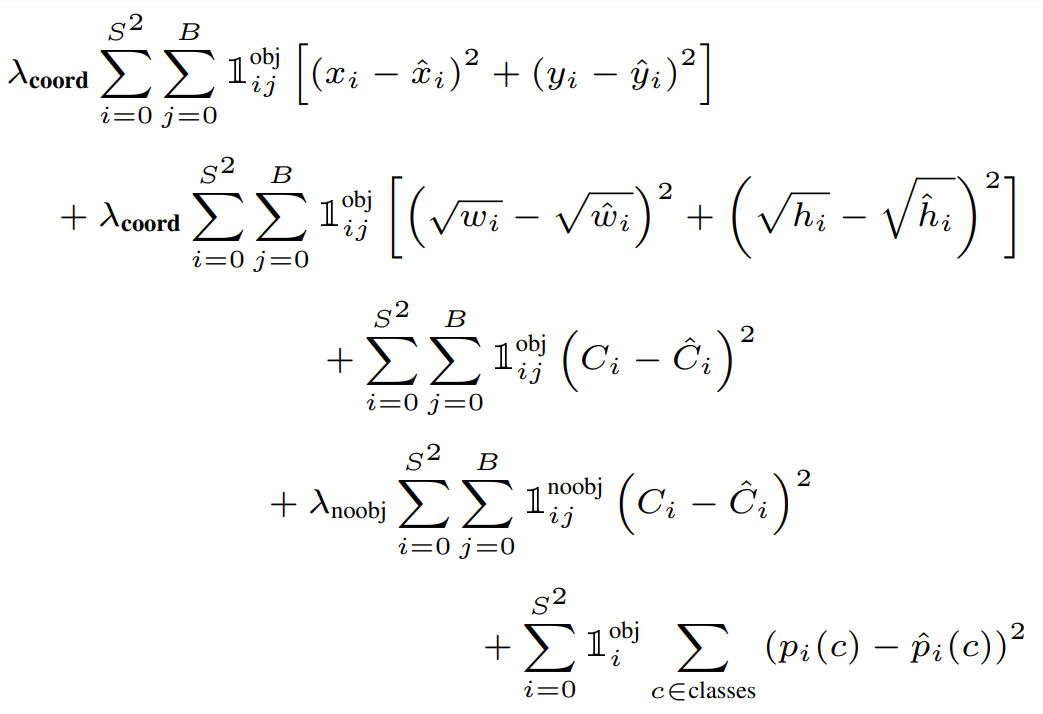
\includegraphics[width=0.4\textwidth]{figures/YOLO_Loss.png}
    \caption{YOLOv1 Loss function ~\cite{YOLO_OG}}
    \label{fig:YOLO_Loss}
\end{figure}\\
YOLOv1 uses stochastic gradient descent as its optimizer; the Loss function is shown in Fig. 1. The Loss function comprises two parts, localization loss, and classification loss. The localization loss measures the error between the predicted bounding box coordinates and the ground-truth bounding box. The classification loss measures the error between the predicted class probabilities and the ground truth. The $\lambda_{coord}$ and $\lambda_{noobj}$ are regularization coefficients that regulate the magnitude of the different components, emphasizing object localization and deemphasizing grid cells without objects.\\

\subsection{YOLOv5 Overview}
YOLOv5 is an object detection model that was first introduced in 2020 by Ultralytics, which builds on the success of previous YOLO models. YOLOv5 achieved SOTA performance on a variety of benchmark datasets while also being fast and efficient to train and deploy. YOLO made several architectural changes when YOLOv5 came around, most notably the standardized practice of structuring the model into three components, the backbone, the neck, and the head.\\
\begin{figure}[h]
    \centering
    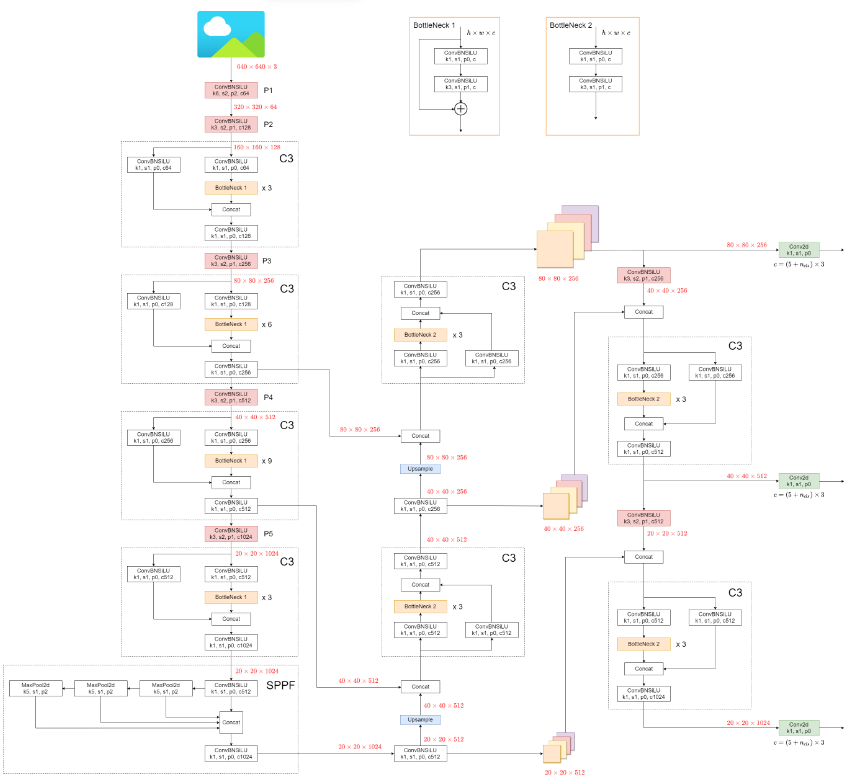
\includegraphics[width=0.4\textwidth]{figures/YOLOv5_arch.png}
    \caption{YOLOv5 Architecture}
    \label{fig:my_label}
\end{figure} 
The backbone of YOLOv5 is a variant of Darknet53, a new network for performing feature extraction characterized by small filter windows and residual connections. YOLOv5 modifies Darknet 53 by introducing Cross Stage Partial (CSP) connections to the network. This enables the architecture to achieve a richer gradient combination while reducing the amount of computation. It involves dividing the backbone into two streams, one processing the image and another which processes a downsampled version of the input. They are later concatenated and passed to the next stage of the network. \\
The neck of YOLOv5 is the Intermediate component that connects the backbone to the head. It aggregates and refines the features extracted by the backbone, often focusing on enhancing the spatial and semantic information across different scales. \\
The first half of the neck is composed of a Spatial Pyramid Pooling (SPP) layer to remove the fixed-size constraint of the network, which is typically a requirement due to the final fully connected layers during the inference phase. This removes the need to warp, augment, or crop images, which generally change the aspect ratio and scale of the object in the image. \\
The second half of the neck, the CSP-Path Aggregation Network (CSP-PAN), incorporates the features learned by the CSP blocks in the backbone and shortens the information path between lower layers and top features. PAN links the feature grid and all feature levels to make helpful information in each feature level propagate directly to subblocks. \\
YOLOv5’s head consists of three branches, each predicting a different feature scale. In the original publication, the authors used different grid cell shapes for each level, especially grid cell sizes of 13 x 13, 26 x 26, and 52 x 52, with each grid cell predicting B = 3 bounding boxes. Each head produces bounding boxes, class probabilities, and confidence scores, with the output tensor being of shape S x S x (B x 5 + C), where 5 represents x, y, w, h, and the confidence score of the predicted class. Finally, the network uses Non-maximum Suppression (NMS) to filter out overlapping bounding boxes and only keep the most confident predictions.\\
YOLOv5 also incorporates anchor boxes, fixed-sized bounding boxes used to predict the location and size of objects within an image. Instead of predicting arbitrary bounding boxes for each object instance, the model predicts the coordinates of the anchor boxes with predefined aspect ratios and scales and adjusts them to fit the object instance.\\

\subsection{YOLOv8 Overview}
YOLOv8 is the latest version of the YOLO object detection model. This latest version has the same architecture as its predecessors \ref{fig:YOLOv8_arch} but it introduces numerous improvements compared to the earlier versions of YOLO such as a new neural network architecture that utilizes both Feature Pyramid Network (FPN) and Path Aggregation Network (PAN) and a new labeling tool that simplifies the annotation process. This labeling tool contains several useful features like auto labeling, labeling shortcuts, and customizable hotkeys. The combination of these features makes it easier to annotate images for training the model.
\begin{figure}[h]
    \centering
    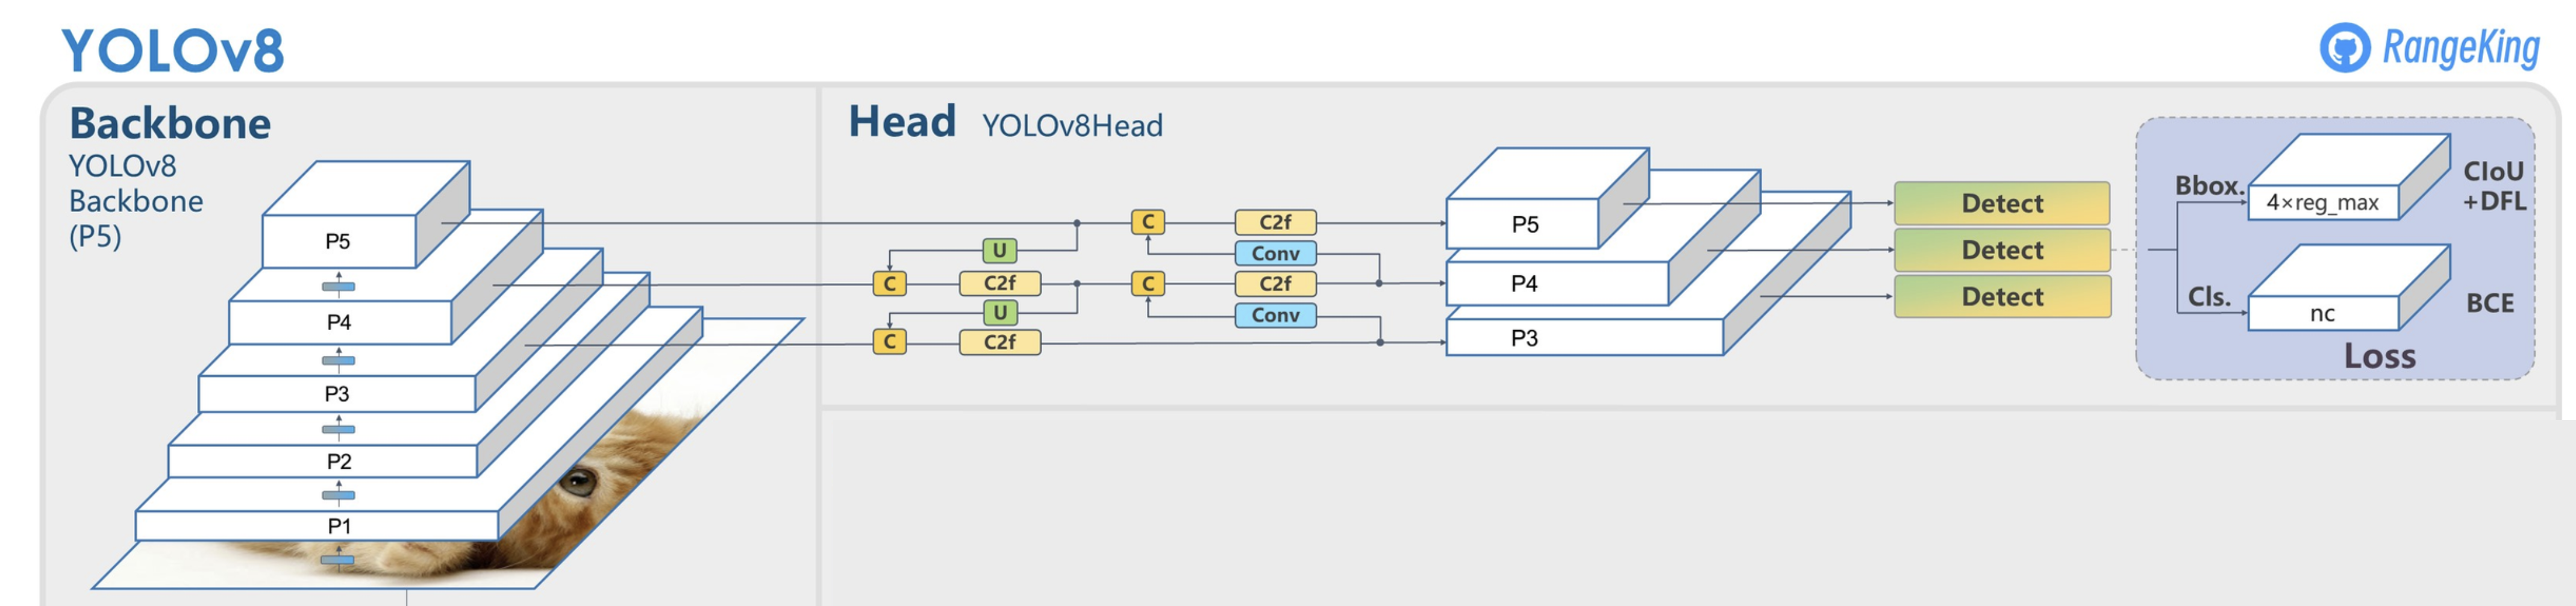
\includegraphics[width=0.4\textwidth]{figures/YOLOv8_arch.png}
    \caption{YOLOv8 Architecture ~\cite{YOLOv8Website}}
    \label{fig:YOLOv8_arch}
\end{figure}
\\
The FPN works by gradually reducing the spatial resolution of the input image while increasing the number of feature channels. This results in the creation of feature maps that are capable of detecting objects at different scales and resolutions. The PAN architecture, on the other hand, aggregates features from different levels of the network through skip connections. By doing so, the network can better capture features at multiple scales and resolutions, which is crucial for accurately detecting objects of different sizes and shapes ~\cite{CompReview}\\

\subsection{YOLOv8 vs YOLOv5}
The reason YOLOv8 is being compared to YOLOv5 and not any other version of YOLO is that YOLOv5’s performance and metrics are closer to YOLOv8’s. However, YOLOv8 surpasses YOLOv5 in aspects including a better mAP as seen in Figure \ref{fig:YOLOv8_mAP}. Along with a better mAP, this shows that YOLOv8 has fewer outliers when measured against the RF100 which is a 100-sample dataset from the Roboflow universe which is a repository of 100,000 datasets. We also witness YOLOv8 outperforming YOLOv5 for each RF100 category. From the Figure \ref{fig:YOLOv8_average_mAP_against_cats} we can see that YOLOv8 produces similar or even better results compared to YOLOv5 ~\cite{YOLOv8Website}.
\begin{figure}[h]
    \centering
    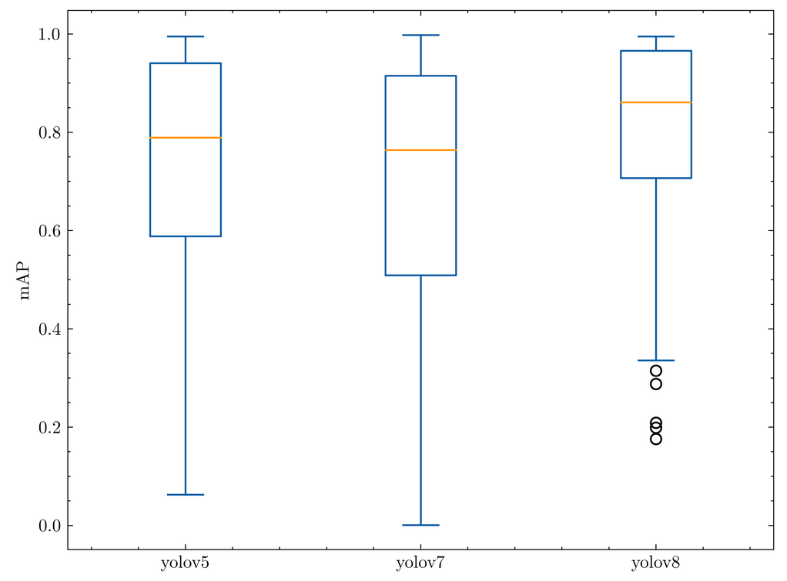
\includegraphics[width=0.4\textwidth]{figures/YOLOv5_vs_YOLOv8_COMP1.png}
    \caption{YOLOs mAP@.50 against RF100 ~\cite{YOLOv8Website}}
    \label{fig:YOLOv8_mAP}
\end{figure}
\begin{figure}[h]
    \centering
    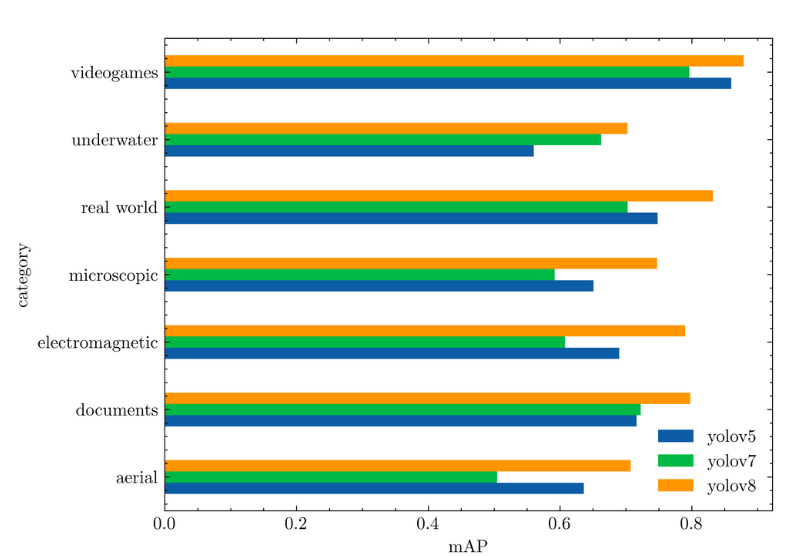
\includegraphics[width=0.4\textwidth]{figures/YOLOv5_vs_YOLOv8_COMP2.png}
    \caption{YOLOs average mAP@.50 against RF100 categories ~\cite{YOLOv8Website}}
    \label{fig:YOLOv8_average_mAP_against_cats}
\end{figure}
\\
As mentioned previously, YOLOv8 uses a new architecture that combines both FAN and PAN modules. FPN is used to generate feature maps at multiple scales and resolutions, while PAN is used to aggregate features from different levels of the network to improve accuracy. The results of the combined FAN and PAN modules are better than YOLOv5 which uses a modified version of CSPDarknet architecture. This modified version of CSPDarknet is based off the cross-stage partial connections (CSP), which improves the flow of information between different parts of the network.\\  
Another difference the two models have is their training data. YOLOv8 was trained on a larger and more diverse dataset compared to YOLOv5. YOLOv8 was trained on a blend of the COCO dataset and several other datasets, while YOLOv5 was trained primarily on the COCO dataset. Because of that, YOLOv8 has a better performance on a wider range of images.\\
YOLOv8 includes a new labeling tool called RoboFlow Annotate which is used for image annotation and object detection tasks in computer vision. RoboFlow Annotate makes it easier to annotate images for training the model and includes several features such as auto labeling, labeling shortcuts, and customizable hotkeys. In contrast, YOLOv5 uses a different labeling tool called LabelImg. LabelImg is an open-source graphical image annotation tool that allows its users to draw bounding boxes around objects of interest in an image, and then export the annotations in the YOLO format for training the model.\\
YOLOv8 includes more advanced post-processing techniques than YOLOv5, which are a set of algorithms applied to the predicted bounding boxes and objectiveness scores generated by the neural network. These techniques help to refine the detection results, remove redundant detections, and improve the overall accuracy of the predictions. YOLOv8 uses Soft-NMS which is a variant of the NMS technique used in YOLOv5. Soft-NMS applies a soft threshold to the overlapping bounding boxes instead of discarding them outright. Whereas NMS removes the overlapping bounding boxes and keeps only the ones with the highest objectiveness score.\\		
Output heads refer to the final layers of a neural network that predict the locations and classes of objects in an image. In YOLO architecture there are typically several output heads that are responsible for predicting different aspects of the detected objects, such as the bounding box coordinates, class probabilities, and objectiveness scores. These output heads are typically connected to the last few layers of the neural network and are trained to output a set of values that can be used to localize and classify objects in an image. The number and type of output heads used can vary depending on the specific object detection algorithm and the requirements of the task at hand. YOLOv5 has 3 output heads while YOLOv8 has 1 output head. YOLOv8 Does not have small, medium, and large anchor boxes rather it uses an anchor free detection mechanism that directly predicts the center of an object instead of the offset from a known anchor box which reduces the number of box predictions, and that speeds up the post processing process.\\
It is fair to note that YOLOv8 is slightly slower than YOLOv5 when talking about object detection speed. However, YOLOv8 is still able to process images in real-time on modern GPUs.\\
Both YOLOv5 and YOLOv8 use mosaic augmentation on the training set. Mosaic augmentation is a data augmentation technique that takes four random images from the training set and combines them into a single mosaic image. This image, where each quadrant contains a random crop from one of the four input images, is then inputted into the model ~\cite{MosaicAug}
%---------------------------------------------------------------------
\section{Model Evaluation}

\begin{figure}[h]
    \centering
    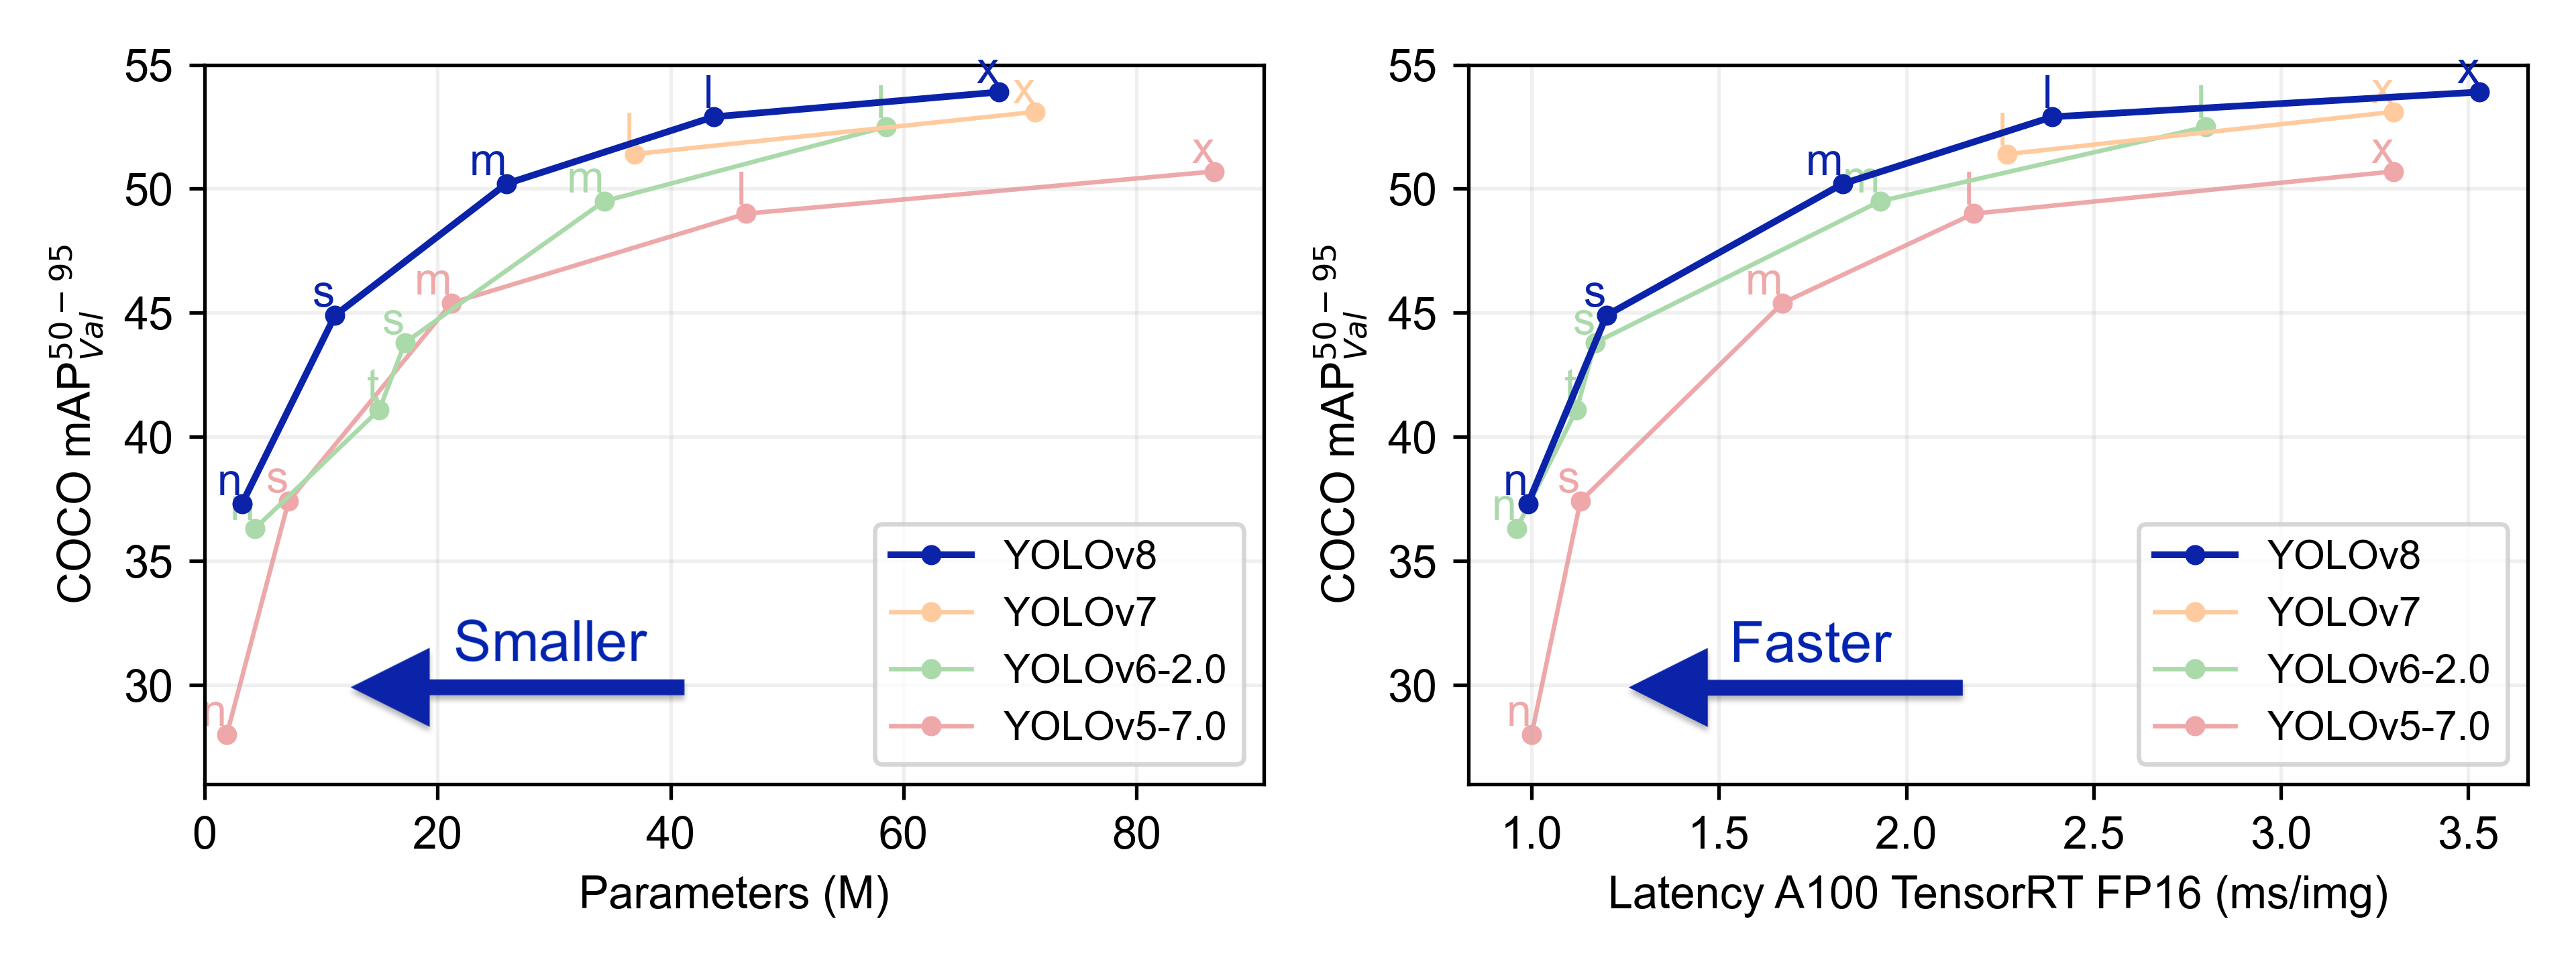
\includegraphics[width=0.45\textwidth]{figures/yolo-comparison-plots.png}
    \caption{Shows the performance of each YOLO model and its respective versions for mAP50 against a number of parameters and inference speed}
    \label{fig:my_label}
\end{figure}

Mean Average Precision (mAP) is a commonly used evaluation metric for object detection that combines Precision, recall, IOU, and AP. Precision is the ratio of true positives to the total number of detections. At the same time, recall is the ratio of true positives to the total number of ground truth objects in an image. Recall values range from 0.0 to 1.0 with a stepsize of 0.1. In contrast, the interpolated precision value is defined as the maximum Precision corresponding to the recall value more significant than the current recall value. The curve we obtain is commonly called the precision-recall curve. Average Precision is therefore defined as the area underneath this curve. A higher AP score indicates better performance since it means the model is accurately detecting more objects in an image while minimizing false positives.\\
It is essential to define what we consider a valid detection by our model. mAP50 uses IoU as its threshold parameter, defined as an area of overlap over an area of union between the predicted bounding box and ground truth, set at an IoU = 50\% or greater. Finally, we average the result APs over all the category classes to obtain mAP50. mAP50:95 corresponds to the average mAP across all categories for different IoU thresholds, starting from 50% to 95%, with a step size of 5\%. This provides a more comprehensive evaluation of the model’s performance across various confidence levels.

% \begin{figure}[h]
%     \centering
%     \subfloat[\centering Confusion matrix for the different classes]{{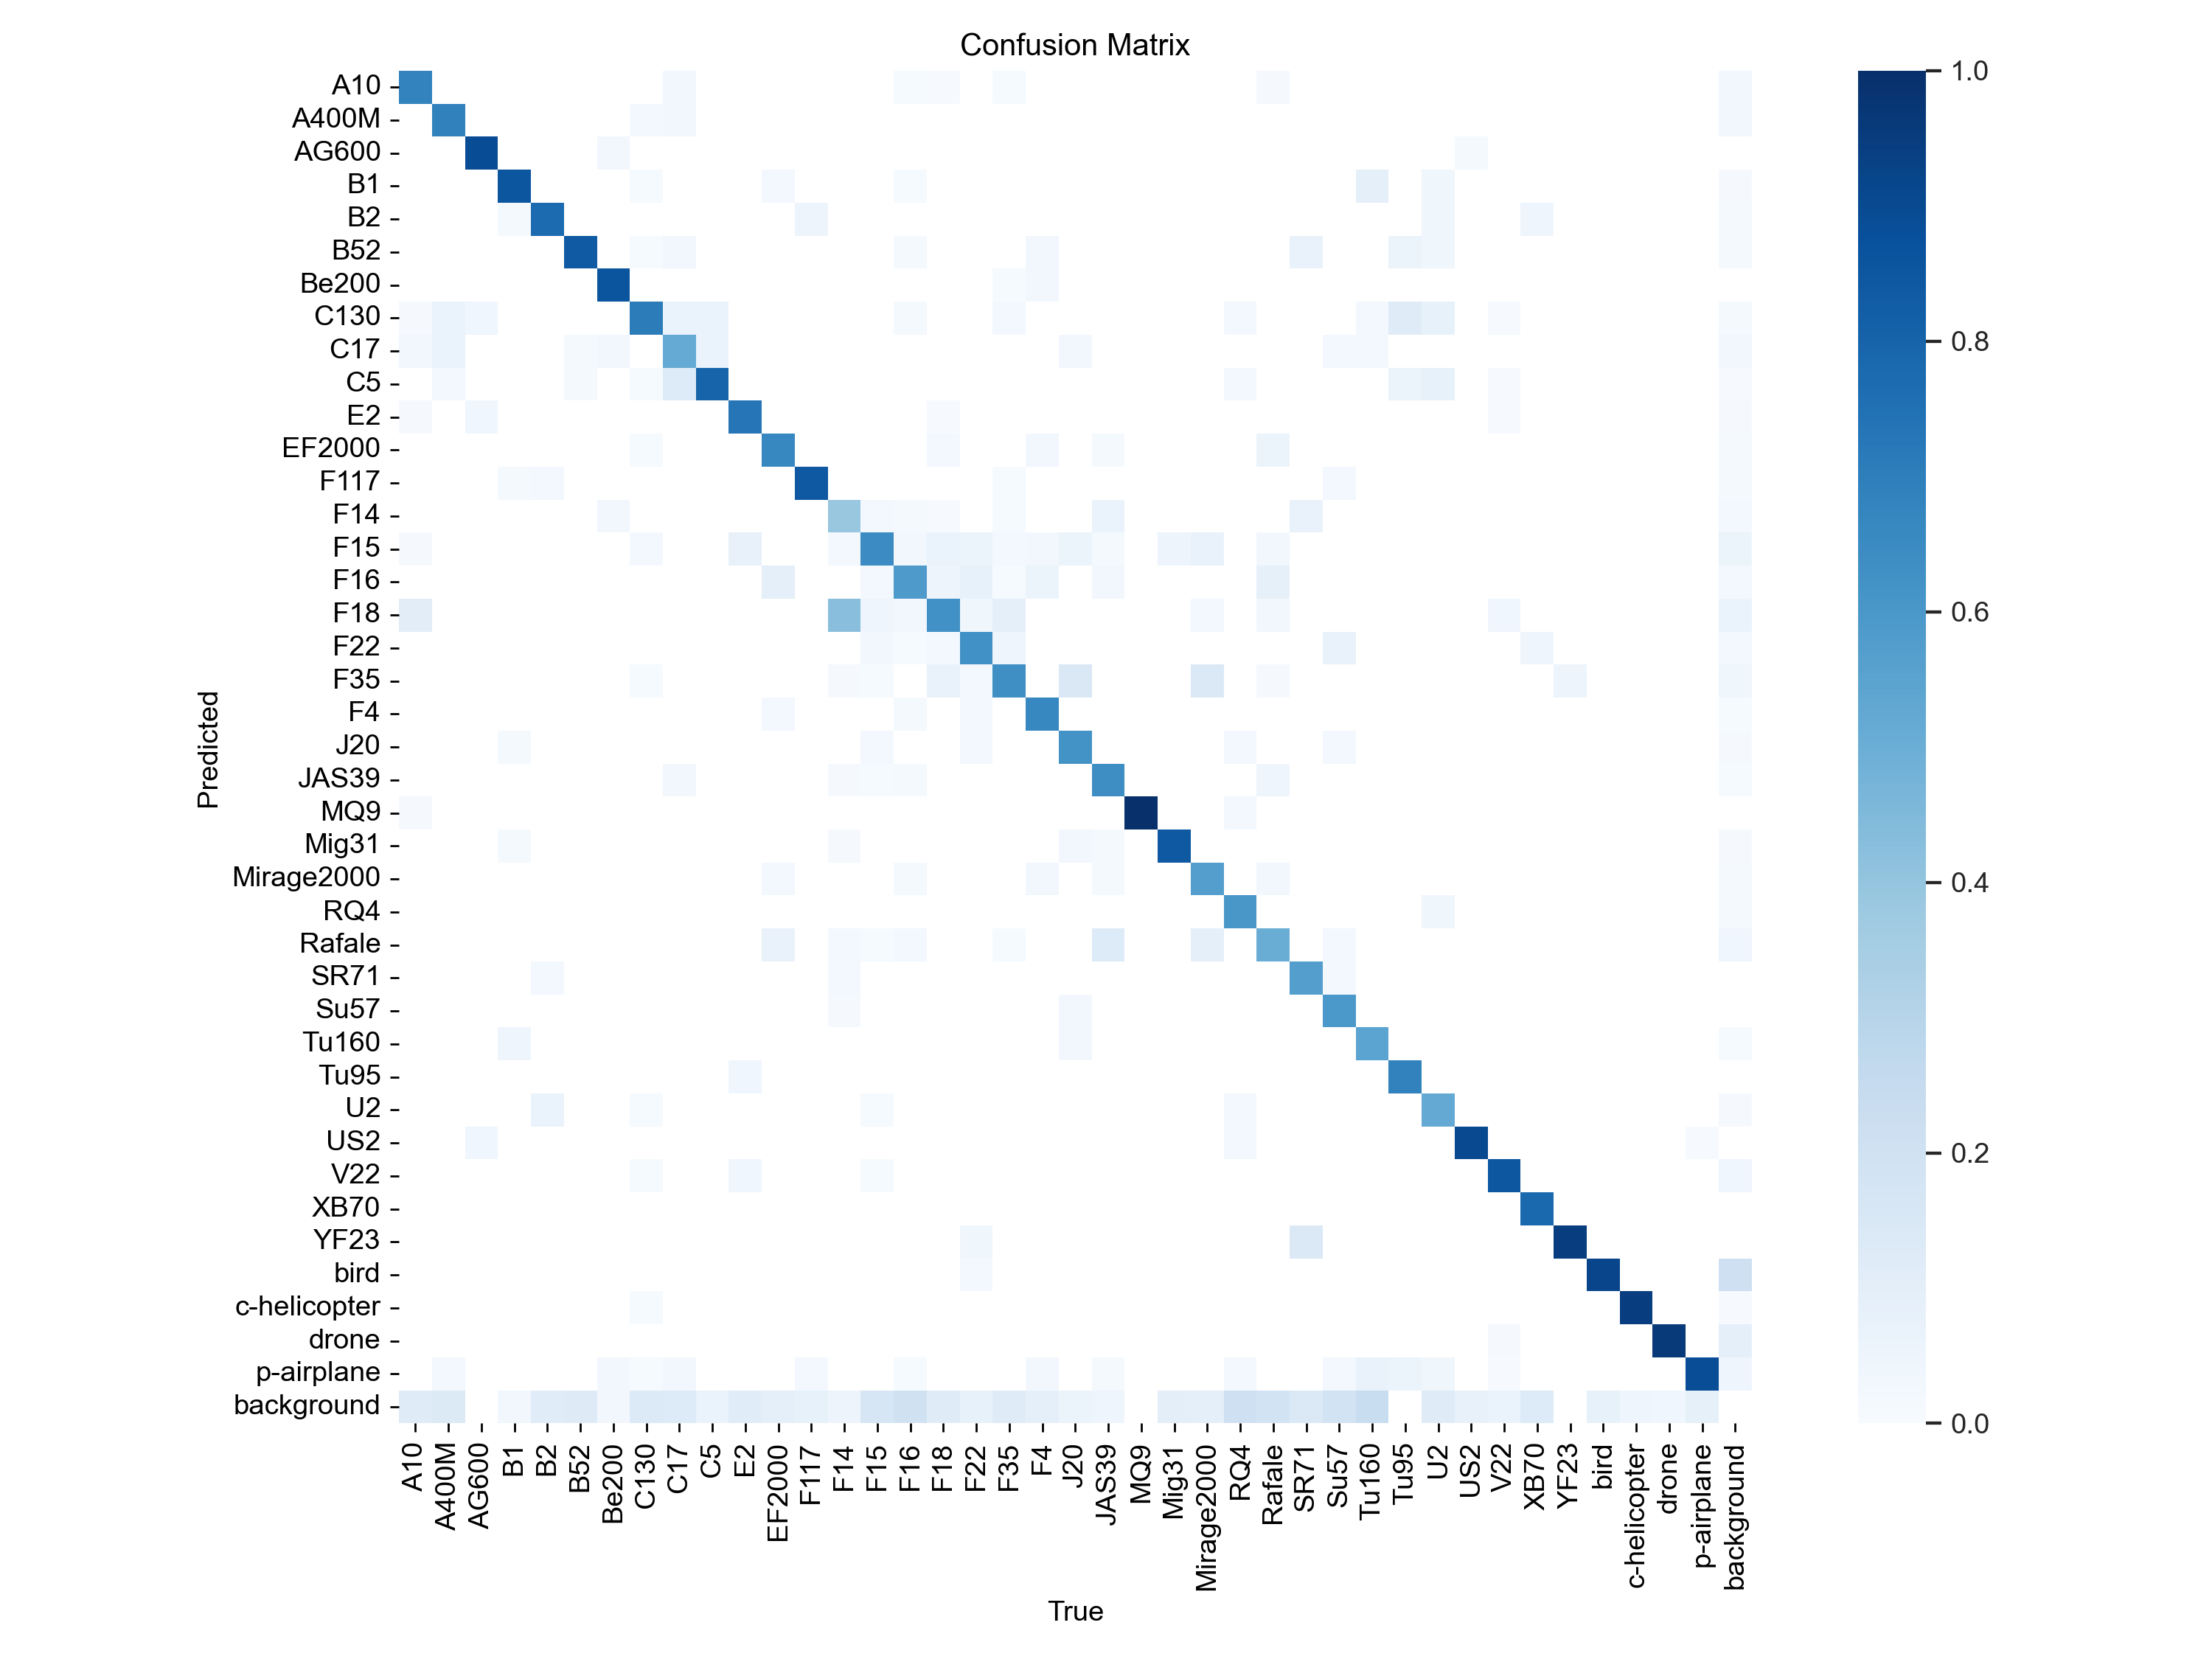
\includegraphics[width=3.2cm]{figures/confusion_matrix.png}}}
%     \qquad
%     \subfloat[\centering PR curve showing for each individual class and overall]{{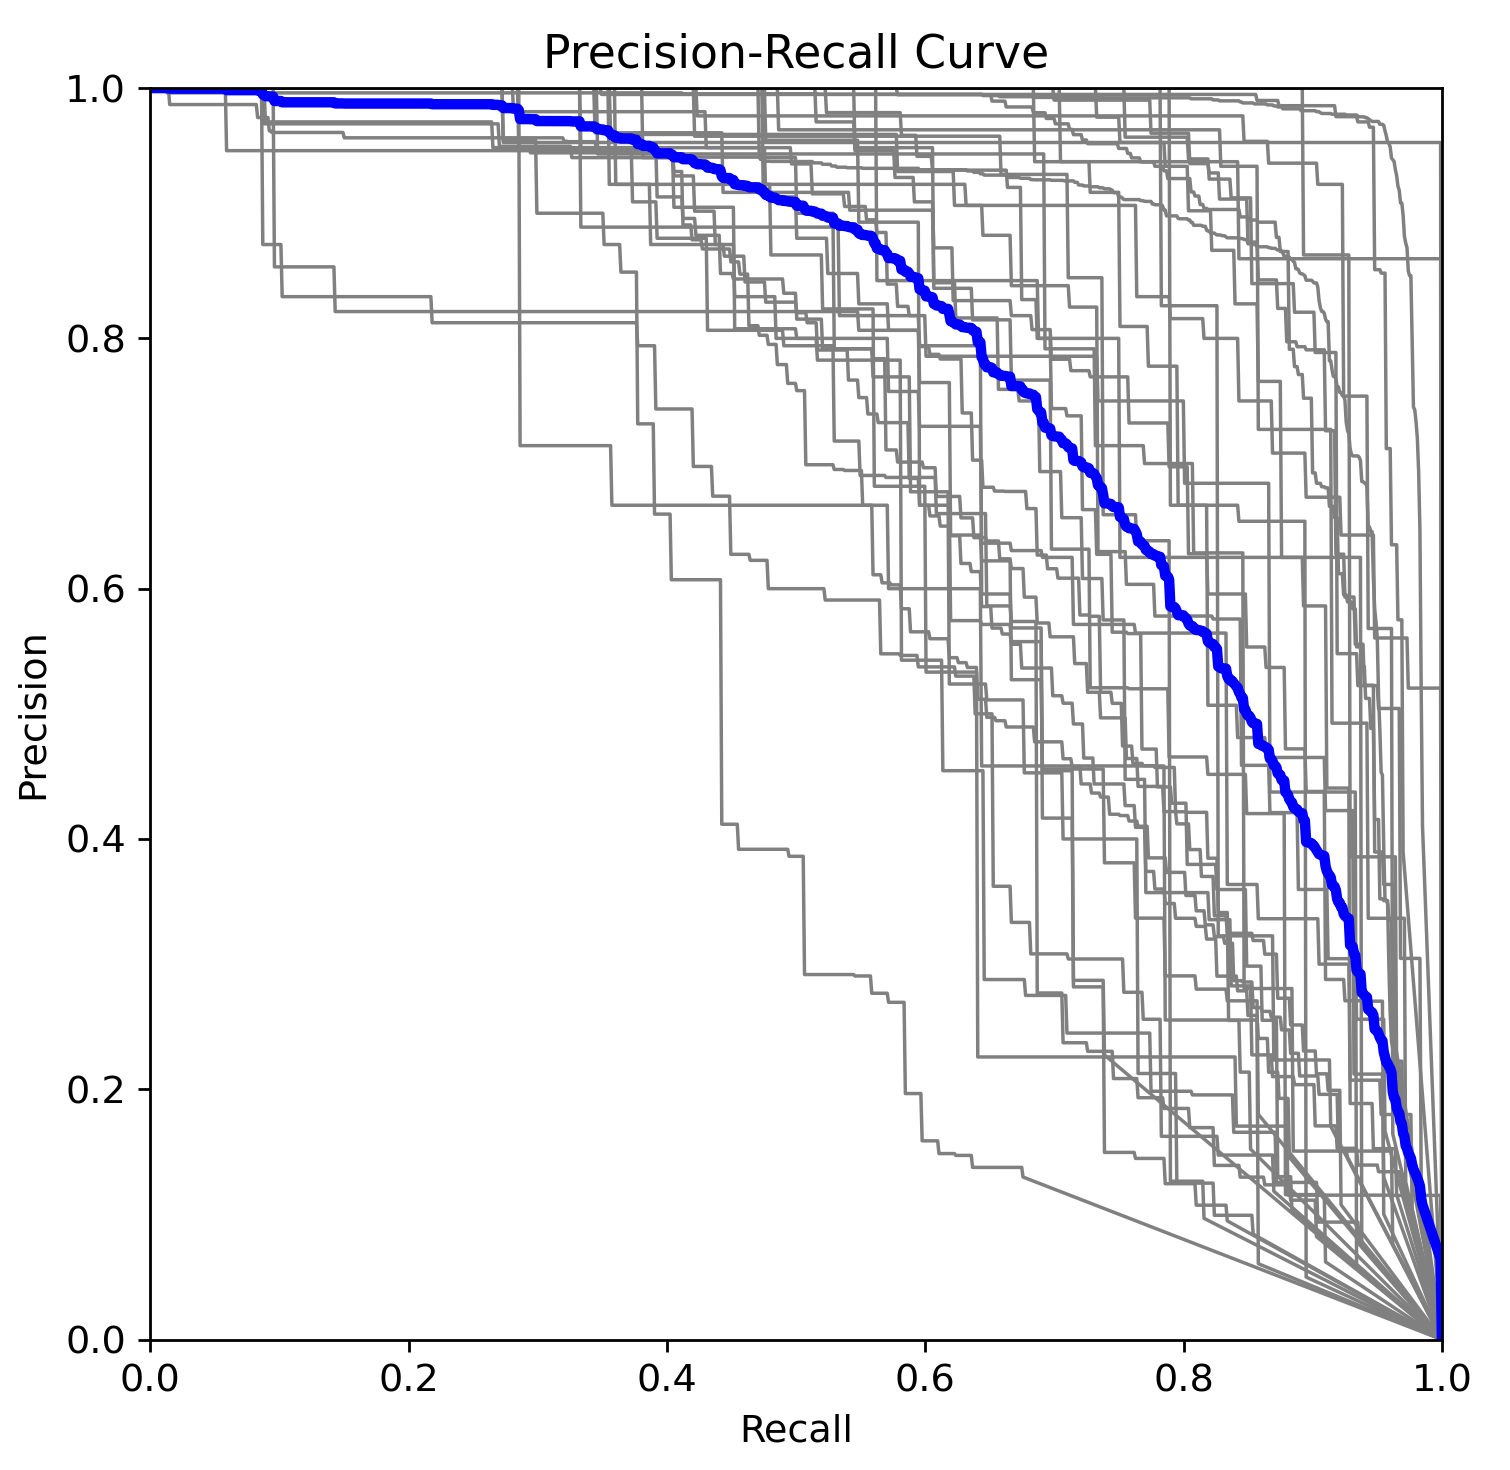
\includegraphics[width=3.5cm]{figures/PR_curve.png} }}%
%     \caption{TBA}%
%     \label{fig:example}
% \end{figure}

The model we performed our evaluation on was the YOLOv8m model, which was trained on the flying object detection dataset, saw a mAP@50 = 79.2\% and mAP@50:95 = 68.5\%. Performance was relatively stable across most classes according to the confusion matrix in Fig. 5. 

\newpage
{\small
\bibliographystyle{ieee_fullname}
\bibliography{egbib}
}

\begin{table*}
\begin{center}
\begin{tabular}{|l|c|p{8cm}|}
\hline
Student Name & Contributed Aspects & Details \\
\hline\hline
Team Member 1 & Data Creation and Implementation & Scraped the dataset for this project and trained the CNN of the encoder. Implemented attention mechanism to improve results. \\
Team Member 2 & Implementation and Analysis & Trained the LSTM of the encoder and analyzed the results. Analyzed effect of number of nodes in hidden state.  Implemented Convolutional LSTM. \\
Team Member 3 & Implementation and Analysis & Trained the LSTM of the encoder and analyzed the results. Analyzed effect of number of nodes in hidden state.  Implemented Convolutional LSTM. \\
Team Member 4 & Implementation and Analysis & Trained the LSTM of the encoder and analyzed the results. Analyzed effect of number of nodes in hidden state.  Implemented Convolutional LSTM. \\
\hline
\end{tabular}
\end{center}
\caption{Contributions of team members.}
\label{tab:contributions}
\end{table*}
\end{document}
						




			  
